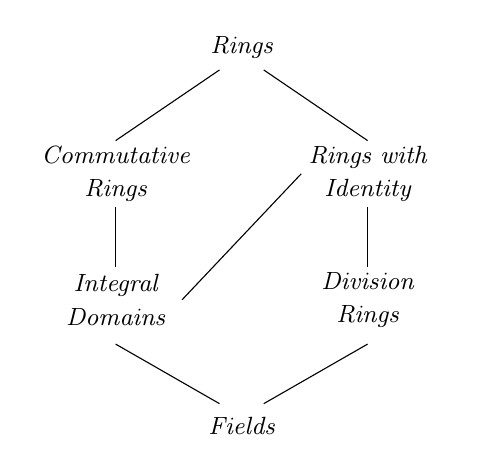
\begin{tikzpicture}[scale=0.8]

\coordinate (rings-label) at (0,3);
\coordinate (commutative-rings-label) at (-2,1);
\coordinate (rings-w-identity-label) at (2,1);
\coordinate (integral-domains-label) at (-2,-1);
\coordinate (division-rings-label) at (2,-1);
\coordinate (fields-label) at (0,-3);

\node at (rings-label) {\small \it Rings};
\node [text width=2cm, text centered] at (commutative-rings-label) {\small \it Commutative Rings};
\node [text width=2cm, text centered] at (rings-w-identity-label) {\small \it Rings with Identity};
\node [text width=1.5cm, text centered] at (integral-domains-label) {\small \it Integral Domains};
\node [text width=1.5cm, text centered] at (division-rings-label) {\small \it Division Rings};
\node at (fields-label) {\small \it Fields};

\draw  ([xshift=-10,yshift=-10]rings-label) -- ([yshift=15]commutative-rings-label);
\draw  ([xshift=10,yshift=-10]rings-label) -- ([yshift=15]rings-w-identity-label);
\draw  ([yshift=-15]commutative-rings-label) -- ([yshift=15]integral-domains-label);
\draw  ([xshift=-30]rings-w-identity-label) -- ([xshift=30]integral-domains-label);
\draw  ([yshift=-15]rings-w-identity-label) -- ([yshift=15]division-rings-label);
\draw  ([yshift=-20]integral-domains-label) -- ([xshift=-10,yshift=10]fields-label);
\draw  ([yshift=-20]division-rings-label) -- ([xshift=10,yshift=10]fields-label);


\end{tikzpicture}
